\documentclass{article}
\usepackage[spanish]{babel} %Definir idioma español
\usepackage[utf8]{inputenc} %Codificacion utf-8
\usepackage{amssymb, amsmath, amsbsy, wasysym}
\usepackage{multirow} % para tablas
\usepackage{graphicx}
\usepackage[dvipsnames]{xcolor}
\title{Práctica 2}
\author{Emmanuel Peto Gutiérrez}
\begin{document}
\maketitle

\section{Introducción}

El problema para esta práctica consiste en encontrar el \textbf{Conjunto Independiente Maximal} dada cualquier gráfica de entrada (No confundir con el Conjunto Independiente de cardinalidad máxima).

Un \textbf{Conjunto Independiente} se define de la siguiente manera: Un conjunto $S$ de vértices de una gráfica es independiente si y sólo si ninguna pareja de vértices en el conjunto $S$ es adyacente. En otras palabras, $S \subseteq V (G)$ es independiente en $G$ si y sólo si la subgráfica inducida por $S$ en $G$ $(G[S])$, no posee aristas.

Ahora bien, un \textbf{Conjunto Independiente Maximal} se trata de un conjunto independiente, tal que si se le agrega cualquier otro vértice al conjunto, éste deja de ser independiente.

\begin{center}
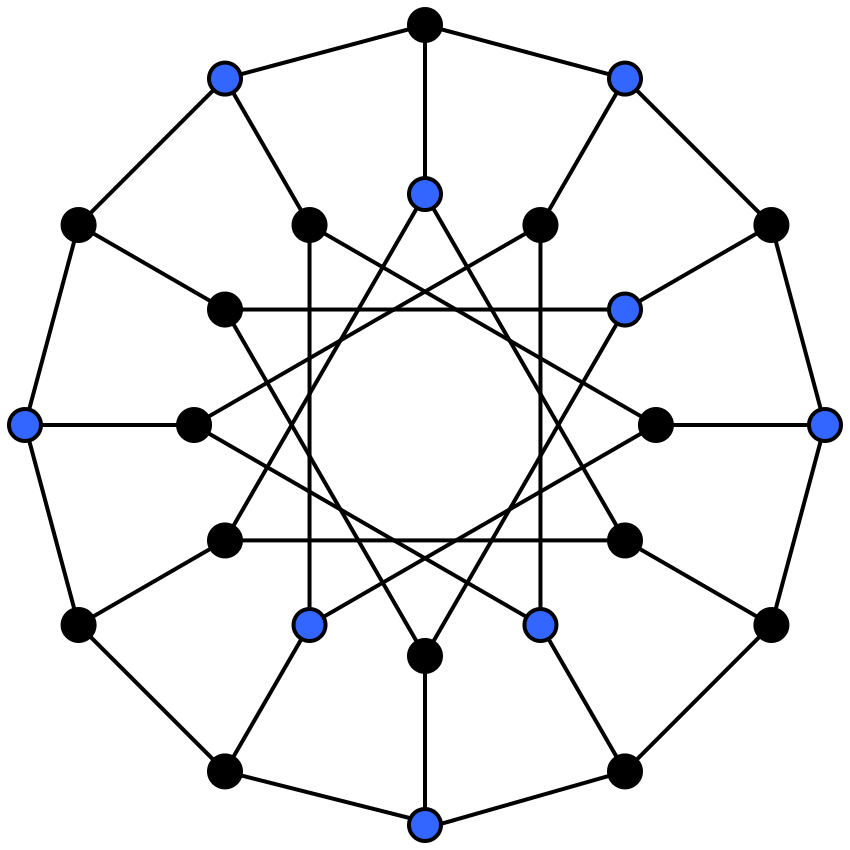
\includegraphics[scale=0.2]{graf1}
\end{center}

Ejemplo de conjunto independiente (Conjunto de vértices azules), es visible que
no existe ninguna arista adyacente a 2 vértices azules.

\begin{center}
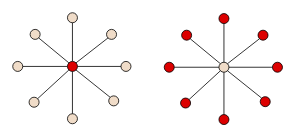
\includegraphics[scale=1]{graf2}
\end{center}

Ejemplo de dos conjuntos independientes maximales para una misma gráfica.

\section{Descripción}

\subsection{Entrada}

El programa a implementar debe recibir como única entrada, en los argumentos
de la linea de comandos, el nombre del \textbf{archivo de texto} que contiene la
información de la gráfica a procesar.

\subsection{Formato}

El archivo de texto de entrada contendrá la información necesaria para encontrar el conjunto independiente en una gráfica. Esto es:

\begin{itemize}
\item En la primer linea, los vértices en la gráfica separados por `,'.
\item De la segunda linea en adelante, pares de vértices separados por `,' que indican las aristas en la gráfica.
\end{itemize}

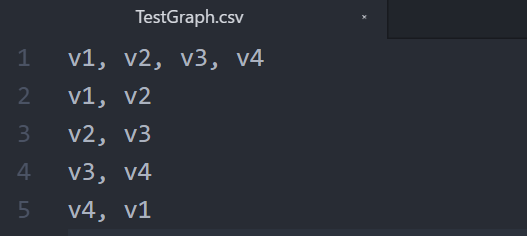
\includegraphics[scale=0.5]{test1}

\subsection{Implementación}

Para esta práctica no está permitido utilizar una matriz de adyacencias para el manejo de la gráfica. El problema debe resolverse utilizando clases que representen a los vértices y la gráfica. Idealmente sólo es necesaria la implementación de 2 clases:

\begin{itemize}
\item Clase Grafica
\item Clase Vertice
\end{itemize}

\subsection{Salida}

La salida del programa debe ser un archivo de texto que contenga los vértices pertenecientes al conjunto independiente maximal encontrado, separados por `,'. El nombre del archivo de salida debe ser:

Salida[NombreArchivoDeEntrada]

Por ejemplo, si el archivo de entrada es ``Amlo.csv'', entonces el archivo de salida debe llamarse ``SalidaAmlo.csv''.

\section{Detalles adicionales}

La práctica debe ser implementada utilizando \textbf{Java}.

Si el programa muestra una representación gráfica del conjunto independiente encontrado, será considerado para complementar la calificación final de sus prácticas.

\section{Entrega}

\begin{itemize}
\item Deben entregarlo como un archivo comprimido de una carpeta con el mismo nombre.
\item La carpeta debe ser: \textbf{Practica2\_ApellidopaternoApellidomaterno}. Por ejemplo \textbf{Practica2\_PetoGutierrez}.
\item Su carpeta debe contener un archivo \emph{readme} que contenga: número de cuenta, nombre completo, 
correo y las instrucciones para compilar y ejecutar su programa(se recomienda un \emph{Makefile}).
\item Si su carpeta contiene un ejecutable(como *.jar) enviarlo como un enlace de dropbox o drive.
\item El asunto debe ser: \textbf{[AAlgoritmos]Practica2}.
\end{itemize}

\end{document}